% Options for packages loaded elsewhere
\PassOptionsToPackage{unicode}{hyperref}
\PassOptionsToPackage{hyphens}{url}
\documentclass[
]{article}
\usepackage{xcolor}
\usepackage{amsmath,amssymb}
\setcounter{secnumdepth}{5}
\usepackage{iftex}
\ifPDFTeX
  \usepackage[T1]{fontenc}
  \usepackage[utf8]{inputenc}
  \usepackage{textcomp} % provide euro and other symbols
\else % if luatex or xetex
  \usepackage{unicode-math} % this also loads fontspec
  \defaultfontfeatures{Scale=MatchLowercase}
  \defaultfontfeatures[\rmfamily]{Ligatures=TeX,Scale=1}
\fi
% \usepackage{lmodern}
\ifPDFTeX\else
  % xetex/luatex font selection
\fi
% Use upquote if available, for straight quotes in verbatim environments
\IfFileExists{upquote.sty}{\usepackage{upquote}}{}
\IfFileExists{microtype.sty}{% use microtype if available
  \usepackage[]{microtype}
  \UseMicrotypeSet[protrusion]{basicmath} % disable protrusion for tt fonts
}{}
\makeatletter
\@ifundefined{KOMAClassName}{% if non-KOMA class
  \IfFileExists{parskip.sty}{%
    \usepackage{parskip}
  }{% else
    \setlength{\parindent}{0pt}
    \setlength{\parskip}{6pt plus 2pt minus 1pt}}
}{% if KOMA class
  \KOMAoptions{parskip=half}}
\makeatother
\usepackage{color}
\usepackage{fancyvrb}
\newcommand{\VerbBar}{|}
\newcommand{\VERB}{\Verb[commandchars=\\\{\}]}
\DefineVerbatimEnvironment{Highlighting}{Verbatim}{commandchars=\\\{\}}
% Add ',fontsize=\small' for more characters per line
\newenvironment{Shaded}{}{}
\newcommand{\AlertTok}[1]{\textcolor[rgb]{1.00,0.00,0.00}{\textbf{#1}}}
\newcommand{\AnnotationTok}[1]{\textcolor[rgb]{0.38,0.63,0.69}{\textbf{\textit{#1}}}}
\newcommand{\AttributeTok}[1]{\textcolor[rgb]{0.49,0.56,0.16}{#1}}
\newcommand{\BaseNTok}[1]{\textcolor[rgb]{0.25,0.63,0.44}{#1}}
\newcommand{\BuiltInTok}[1]{\textcolor[rgb]{0.00,0.50,0.00}{#1}}
\newcommand{\CharTok}[1]{\textcolor[rgb]{0.25,0.44,0.63}{#1}}
\newcommand{\CommentTok}[1]{\textcolor[rgb]{0.38,0.63,0.69}{\textit{#1}}}
\newcommand{\CommentVarTok}[1]{\textcolor[rgb]{0.38,0.63,0.69}{\textbf{\textit{#1}}}}
\newcommand{\ConstantTok}[1]{\textcolor[rgb]{0.53,0.00,0.00}{#1}}
\newcommand{\ControlFlowTok}[1]{\textcolor[rgb]{0.00,0.44,0.13}{\textbf{#1}}}
\newcommand{\DataTypeTok}[1]{\textcolor[rgb]{0.56,0.13,0.00}{#1}}
\newcommand{\DecValTok}[1]{\textcolor[rgb]{0.25,0.63,0.44}{#1}}
\newcommand{\DocumentationTok}[1]{\textcolor[rgb]{0.73,0.13,0.13}{\textit{#1}}}
\newcommand{\ErrorTok}[1]{\textcolor[rgb]{1.00,0.00,0.00}{\textbf{#1}}}
\newcommand{\ExtensionTok}[1]{#1}
\newcommand{\FloatTok}[1]{\textcolor[rgb]{0.25,0.63,0.44}{#1}}
\newcommand{\FunctionTok}[1]{\textcolor[rgb]{0.02,0.16,0.49}{#1}}
\newcommand{\ImportTok}[1]{\textcolor[rgb]{0.00,0.50,0.00}{\textbf{#1}}}
\newcommand{\InformationTok}[1]{\textcolor[rgb]{0.38,0.63,0.69}{\textbf{\textit{#1}}}}
\newcommand{\KeywordTok}[1]{\textcolor[rgb]{0.00,0.44,0.13}{\textbf{#1}}}
\newcommand{\NormalTok}[1]{#1}
\newcommand{\OperatorTok}[1]{\textcolor[rgb]{0.40,0.40,0.40}{#1}}
\newcommand{\OtherTok}[1]{\textcolor[rgb]{0.00,0.44,0.13}{#1}}
\newcommand{\PreprocessorTok}[1]{\textcolor[rgb]{0.74,0.48,0.00}{#1}}
\newcommand{\RegionMarkerTok}[1]{#1}
\newcommand{\SpecialCharTok}[1]{\textcolor[rgb]{0.25,0.44,0.63}{#1}}
\newcommand{\SpecialStringTok}[1]{\textcolor[rgb]{0.73,0.40,0.53}{#1}}
\newcommand{\StringTok}[1]{\textcolor[rgb]{0.25,0.44,0.63}{#1}}
\newcommand{\VariableTok}[1]{\textcolor[rgb]{0.10,0.09,0.49}{#1}}
\newcommand{\VerbatimStringTok}[1]{\textcolor[rgb]{0.25,0.44,0.63}{#1}}
\newcommand{\WarningTok}[1]{\textcolor[rgb]{0.38,0.63,0.69}{\textbf{\textit{#1}}}}
\usepackage{longtable,booktabs,array}
\newcounter{none} % for unnumbered tables
\usepackage{calc} % for calculating minipage widths
% Correct order of tables after \paragraph or \subparagraph
\usepackage{etoolbox}
\makeatletter
\patchcmd\longtable{\par}{\if@noskipsec\mbox{}\fi\par}{}{}
\makeatother
% Allow footnotes in longtable head/foot
\IfFileExists{footnotehyper.sty}{\usepackage{footnotehyper}}{\usepackage{footnote}}
\makesavenoteenv{longtable}
\usepackage{graphicx}
\makeatletter
\newsavebox\pandoc@box
\newcommand*\pandocbounded[1]{% scales image to fit in text height/width
  \sbox\pandoc@box{#1}%
  \Gscale@div\@tempa{\textheight}{\dimexpr\ht\pandoc@box+\dp\pandoc@box\relax}%
  \Gscale@div\@tempb{\linewidth}{\wd\pandoc@box}%
  \ifdim\@tempb\p@<\@tempa\p@\let\@tempa\@tempb\fi% select the smaller of both
  \ifdim\@tempa\p@<\p@\scalebox{\@tempa}{\usebox\pandoc@box}%
  \else\usebox{\pandoc@box}%
  \fi%
}
% Set default figure placement to htbp
\def\fps@figure{htbp}
\makeatother
\setlength{\emergencystretch}{3em} % prevent overfull lines
\providecommand{\tightlist}{%
  \setlength{\itemsep}{0pt}\setlength{\parskip}{0pt}}
\usepackage[]{natbib}
\bibliographystyle{plainnat}
\makeatletter
\@ifpackageloaded{subcaption}{}{\usepackage{subcaption}}
\@ifpackageloaded{caption}{}{\usepackage{caption}}
\captionsetup[subfigure]{margin=0.5em}
\AtBeginDocument{%
\renewcommand*\figurename{Figure}
\renewcommand*\tablename{Table}
}
\AtBeginDocument{%
\renewcommand*\listfigurename{List of Figures}
\renewcommand*\listtablename{List of Tables}
}
\newcounter{pandoccrossref@subfigures@footnote@counter}
\newenvironment{pandoccrossrefsubfigures}{%
\setcounter{pandoccrossref@subfigures@footnote@counter}{0}
\begin{figure}\centering%
\gdef\global@pandoccrossref@subfigures@footnotes{}%
\DeclareRobustCommand{\footnote}[1]{\footnotemark%
\stepcounter{pandoccrossref@subfigures@footnote@counter}%
\ifx\global@pandoccrossref@subfigures@footnotes\empty%
\gdef\global@pandoccrossref@subfigures@footnotes{{##1}}%
\else%
\g@addto@macro\global@pandoccrossref@subfigures@footnotes{, {##1}}%
\fi}}%
{\end{figure}%
\addtocounter{footnote}{-\value{pandoccrossref@subfigures@footnote@counter}}
\@for\f:=\global@pandoccrossref@subfigures@footnotes\do{\stepcounter{footnote}\footnotetext{\f}}%
\gdef\global@pandoccrossref@subfigures@footnotes{}}
\@ifpackageloaded{float}{}{\usepackage{float}}
\floatstyle{ruled}
\@ifundefined{c@chapter}{\newfloat{codelisting}{h}{lop}}{\newfloat{codelisting}{h}{lop}[chapter]}
\floatname{codelisting}{Listing}
\newcommand*\listoflistings{\listof{codelisting}{List of Listings}}
\makeatother
\usepackage{bookmark}
\IfFileExists{xurl.sty}{\usepackage{xurl}}{} % add URL line breaks if available
\urlstyle{same}
% fallback for those not using the hyperref driver hyperxmp:
\makeatletter
\@ifundefined{xmpquote}{\newcommand{\xmpquote}[1]{#1}}{}
\makeatother
\hypersetup{
  colorlinks=true,linkcolor=red,urlcolor=red,citecolor=red,anchorcolor=red,filecolor=red,
  pdfcreator={LaTeX via pandoc}}

\author{}
\date{}

\IfFileExists{seqsplit.sty}{\usepackage{seqsplit}}{\newcommand{\seqsplit}[1]{#1}}
\protected\def\breakseq#1{\seqsplit{#1}}
\protected\def\breaktt#1{\begingroup\ttfamily\seqsplit{#1}\endgroup}
\title{A Deterministic Testbed for Self-Organizing Agent-Team Coordination}
\author{Daniel Ari Friedman\\\footnotesize{Active Inference Institute}\\\footnotesize{\texttt{daniel@activeinference.institute}}\\\footnotesize{\href{https://orcid.org/0000-0001-6232-9096}{ORCID: 0000-0001-6232-9096}} \\ \footnotesize{DOI: \href{https://doi.org/10.5281/zenodo.20533669}{10.5281/zenodo.20533669}}}
\date{2026-06-26}

% Core mathematics
\usepackage{amsmath}
\usepackage{amssymb}
\usepackage{amsfonts}

% Document layout
\usepackage{geometry}
\geometry{margin=0.5in}
\usepackage{float}
\usepackage{graphicx}

% Tables
\usepackage{booktabs}
\usepackage{longtable}
\usepackage{array}

% Algorithm typesetting (for pseudocode in the Methodology)
\usepackage[ruled,vlined,linesnumbered]{algorithm2e}

% Code listings
\usepackage{listings}

% Typography and formatting
\usepackage{microtype}
\usepackage{xcolor}

% Cross-references and citations
\usepackage{hyperref}
\hypersetup{
    colorlinks=true,
    allcolors=blue
}
\usepackage[capitalise,noabbrev]{cleveref}
\usepackage{natbib}

\begin{document}

\begin{titlepage}
\centering
\vspace*{2cm}
{\LARGE\bfseries A Deterministic Testbed for Self-Organizing Agent-Team Coordination\par}
\vspace{0.75em}
{\large Ablatable Mechanisms and Measurable Noise-Robustness under a Matched Experiment Budget\par}
\vfill
\makeatletter
{\@author\par}
\vspace{1em}
{\@date\par}
\makeatother
\vfill
\end{titlepage}
\thispagestyle{empty}
\tableofcontents
\newpage


\section{Abstract}\label{sec:abstract}

Recent work on \emph{AutoScientists} \citep{gao2026autoscientists}
coordinates self-organizing teams of language-model agents through a
small set of shared mechanisms: a champion-and-experiment-log shared
state, a registry of retired dead-end directions, effect-size ranking of
candidate directions, noise-band confirmation of claimed improvements,
and stagnation-driven reorganization of teams. This exemplar provides a
deterministic, standalone reference implementation of those mechanisms
and studies them honestly as a \emph{testbed} rather than as a
performance claim.

We make the comparison fair by holding the total number of objective
evaluations fixed: coordinated teams \emph{partition} a single
sequential experiment budget rather than adding parallel compute. Under
that matched budget, coordination cannot --- and in our results does not
--- beat a single-thread baseline on the final champion metric; we
report the actual numbers and claim no speedup. What the testbed
\emph{does} demonstrate are two distinct, independently measurable
benefits. First, noise-robustness: because the objective is stochastic,
a single observed gain can be a draw of evaluation noise, so we separate
the \emph{reported} champion metric from the \emph{clean} noise-free
ground truth and show that noise-band confirmation shrinks the gap
between them by roughly an order of magnitude --- with confirmation on,
the final champion's reported metric sits \(0.0012\) above its clean
value, against \(0.0156\) with confirmation removed, while every
configuration reaches the same clean optimum. Second, search hygiene:
the dead-end registry, consulted by the proposer, cuts redundant
re-probes of retired directions from \(36\) to \(0\) and halts at \(36\)
of the \(60\) experiments --- the same clean answer, reached with less
waste. A per-mechanism ablation isolates each component's contribution,
and the language-model proposer is a clean plug-in seam: a deterministic
rule-based agent drives the reproducible figures, and a live Hermes
agent (served by Ollama) can be swapped in without touching the
coordination loop.

\newpage

\section{Introduction}\label{sec:introduction}

\subsection{Motivation}\label{motivation}

Long-running scientific experimentation --- tuning a model, searching a
design space, optimizing a noisy objective over many trials --- has
become a target for multi-agent language-model systems.
\emph{AutoScientists} \citep{gao2026autoscientists} frames this as a
coordination problem: several agent teams share a running record of what
has been tried, retire directions that repeatedly fail, prioritize
directions with large observed effects, confirm claimed improvements
against evaluation noise, and reorganize when progress stalls. These are
appealing ideas, but they are easy to \emph{describe} and hard to
\emph{attribute}: when a coordinated system performs well, which
mechanism deserves the credit, and how much of an apparent gain is
simply noise?

This exemplar exists to make those questions answerable on a small,
fully reproducible artifact. It is one of a family of research-project
templates in this repository, each pairing a tested computational core
with a rendered manuscript. Here the core is a deterministic
re-implementation of the AutoScientists coordination mechanisms, and the
manuscript is an honest report of what they do.

\subsection{An honest framing}\label{an-honest-framing}

It is tempting to advertise multi-agent coordination as ``faster'' or
``better'' search. We deliberately do not. The decisive design choice in
this testbed is that \textbf{coordinated teams partition the same
sequential experiment budget as the baseline}; they do not add parallel
compute. Splitting a fixed budget across teams is a \emph{constraint},
not extra horsepower. Under such a matched budget there is no mechanism
by which dividing the work can beat doing it in one undivided thread on
the final metric --- and our results confirm that the clean-metric
advantage of coordination over the baseline is exactly zero.

What remains, and what is genuinely worth demonstrating, are two
benefits that the matched budget does \emph{not} foreclose:
\textbf{robustness to evaluation noise} and \textbf{search hygiene}. The
objective is stochastic: every evaluation adds a seeded perturbation, so
an observed ``improvement'' may be a lucky draw rather than a real gain.
We therefore track two quantities throughout:

\begin{itemize}
\tightlist
\item
  the \textbf{reported metric} --- the value the search believes its
  champion achieves, computed from noisy observations; and
\item
  the \textbf{clean metric} --- the noise-free ground-truth value at the
  champion's parameters, available to us only because the objective is
  synthetic.
\end{itemize}

A configuration that accepts noise-inflated champions will show a large
reported-minus-clean gap. Noise-band confirmation is precisely the
mechanism that closes that gap, and the testbed measures by how much.
Separately, we track how the budget is \emph{spent}: the dead-end
registry, consulted by the proposer, lets the search avoid re-probing
directions already known to fail and halt once they are exhausted.
Neither benefit is a speedup --- they change how good the reported
answer is and how much of the budget is wasted, not how good the clean
answer is.

\subsection{Contributions}\label{contributions}

\begin{enumerate}
\def\labelenumi{\arabic{enumi}.}
\tightlist
\item
  \textbf{A deterministic, ablatable reference} for the five
  AutoScientists coordination mechanisms, with every mechanism
  switchable via a single configuration object so its contribution can
  be isolated.
\item
  \textbf{An honest matched-budget comparison} of coordinated teams
  against a single-thread baseline that reports the actual numbers and
  makes no speedup claim.
\item
  \textbf{A reported-vs-clean noise-robustness measurement} that
  quantifies the value of noise-band confirmation as a roughly
  order-of-magnitude reduction in accepted noise.
\item
  \textbf{A search-hygiene measurement} that quantifies the dead-end
  registry as a reduction of redundant re-probes from \(36\) to \(0\)
  and an early halt at \(36\) of \(60\) experiments, with the clean
  optimum unchanged.
\item
  \textbf{A language-model plug-in seam} (\texttt{Proposer} protocol)
  that lets a live Hermes agent replace the deterministic proposer
  without modifying the coordination loop, exercised by an opt-in
  \texttt{requires\_ollama} test.
\end{enumerate}

The remainder of the paper specifies the mechanisms
(sec.~\ref{sec:methodology}), reports the matched-budget comparison and
the per-mechanism ablation with the numbers our scripts actually produce
(sec.~\ref{sec:results}), states the scope and limits of those claims
(sec.~\ref{sec:scope}), and documents reproduction
(sec.~\ref{sec:reproducibility}).

\newpage

\section{Methodology}\label{sec:methodology}

The testbed is a single coordination loop over a fixed budget of
experiments. Each mechanism is an independent module so it can be tested
and ablated in isolation; the loop wires them together. All logic lives
in \texttt{src/}; the analysis scripts only orchestrate, plot, and
write.

\subsection{The synthetic objective}\label{the-synthetic-objective}

The objective stands in for the expensive, stochastic evaluation a real
run would optimize (a validation score, a correlation, a loss). It is a
pure function of \texttt{(params,\ seed)}: identical inputs always yield
identical outputs, which is what makes the whole exemplar reproducible.

For a parameter vector \(x \in \mathbb{R}^d\) with optimum at the
origin, the \textbf{clean} (noise-free) value is

\[
f(x) = -\sum_{i=1}^{d} \left[ x_i^2 + \rho\,\bigl(1 - \cos(2\pi x_i)\bigr) \right],
\]

a smooth global peak at \(x = 0\) (where \(f = 0\)) minus shallow cosine
ripples of amplitude \(\rho\) that create deceptive local optima along
each axis. Higher is better. A single noisy \textbf{observation} adds a
seeded, zero-centred perturbation:

\[
\tilde{f}(x, s) = f(x) + \varepsilon(x, s), \qquad |\varepsilon| \le \sigma_{\text{noise}},
\]

where \(\varepsilon(x, s)\) is derived deterministically from a hash of
the rounded \(x\) and the seed \(s\). Re-evaluating the same point under
a \emph{different} seed gives a different draw (modelling run-to-run
variance); the same seed always reproduces the same value. We use
\(d = 4\), ripple \(\rho = 0.15\), and noise scale
\(\sigma_{\text{noise}} = 0.02\).

\subsection{Shared state}\label{shared-state}

The deterministic core mirrors the AutoScientists shared state: an
immutable \textbf{champion} record \(p^\*\) (parameters, metric,
originating experiment index) plus an append-only \textbf{experiment
log} \(L\) of structured outcomes. Recording an outcome appends it to
\(L\) and promotes the champion only when the outcome \emph{improved}
--- i.e.~it was confirmed and beat the incumbent. The champion metric is
the value plotted against experiment count.

\subsection{The five mechanisms}\label{the-five-mechanisms}

The shared state above underpins all five: every mechanism reads from or
writes to the champion record and the experiment log. The five
\emph{active} coordination mechanisms layered on top of it are
noise-band confirmation, the dead-end registry, effect-size ranking,
stagnation-driven reorganization, and team partitioning. (The abstract
and README count shared state itself as the first of the headline five
and fold team partitioning into reorganization; the two groupings cover
the same machinery --- this section names the coordination \emph{acts},
those entry points name the standing primitive.)

\textbf{Noise-band confirmation.} Because a single observed gain may be
noise, a candidate is confirmed only when its mean metric over several
seeds exceeds the incumbent by more than an empirical noise band. For
seeds \(S\) and per-evaluation noise \(\sigma_{\text{noise}}\), the band
is \(\sigma \cdot \sigma_{\text{noise}} / \sqrt{|S|}\) standard errors
of the mean (default \(\sigma = 2\)), so it shrinks as more seeds are
averaged. A candidate is confirmed iff its mean-over-seeds delta exceeds
the band. This estimator is domain-agnostic; a synchronized generic copy
lives at \breaktt{infrastructure.scientific.confirmation} for reuse.

\textbf{Dead-end registry.} A registry \(D\) keyed by
\breaktt{(axis,\ direction)} tracks consecutive non-improving
experiments. A direction is \emph{retired} after it fails to improve the
champion \texttt{threshold} times in a row (default \(3\)); a confirmed
improvement clears the streak. Agents consult \(D\) before proposing so
exhausted directions are not re-explored. An axis is \emph{fully
retired} only when both its increase and decrease directions are
retired.

\textbf{Effect-size ranking.} The analyst role prioritizes directions
with large observed effects. We estimate each axis's effect size as the
mean absolute metric delta observed for it in \(L\), then order axes by
descending effect --- with the deliberate twist that \textbf{untried
axes sort first}, so under-explored directions are probed before the
search exploits known-large-effect axes. Ties break by axis index for
determinism.

\textbf{Stagnation-driven reorganization.} A detector fires when the
champion has not improved within a window of recent experiments (default
\(10\)). On firing, teams are re-partitioned around the currently
most-promising live axes, dropping fully-retired ones.

\textbf{Team partitioning.} Live axes are dealt round-robin across
\texttt{num\_teams} teams (default \(3\)) so each team works a
complementary slice of the ranked directions. Crucially, the teams share
one budget: experiment \(t\) is taken by team
\(t \bmod \text{num\_teams}\).

\subsection{The coordination loop}\label{the-coordination-loop}

\begin{verbatim}
for each experiment in the budget:
    pick the next team and its live (non-retired) axes
    proposer proposes the next (axis, signed step) from shared state
    evaluate the candidate; if confirmation is on, average over seeds and test the band
    record the outcome; promote the champion if it improved
    update the dead-end registry
    if reorganization is on and the search is stagnant, re-partition teams
\end{verbatim}

Every mechanism is gated by a boolean in \texttt{SearchConfig}. With all
\emph{structural} coordination toggles off and a single team ---
confirmation stays on, so the baseline is itself noise-honest
(sec.~\ref{sec:setup}) --- the loop reduces exactly to the single-thread
baseline, which is what makes the ablation a clean subtraction.

\subsection{The proposer seam}\label{the-proposer-seam}

The loop depends only on a \texttt{Proposer} protocol ---
\texttt{propose(state,\ axes,\ proposer\_id,\ avoid=frozenset())\ -\textgreater{}\ Proposal},
where \texttt{avoid} is the dead-end registry's retired
\breaktt{(axis,\ direction)} pairs so a faithful proposer steers clear of
them. Two \emph{real} implementations are provided (no mocks):

\begin{itemize}
\tightlist
\item
  \textbf{\breaktt{DeterministicProposer}} --- a rule-based policy that
  probes the next assigned axis in the direction that most recently
  improved it, defaulting toward the origin. It drives every rendered
  figure and test.
\item
  \textbf{\texttt{HermesProposer}} --- renders the shared state to a
  prompt, asks a Hermes model (served by Ollama) for the next
  \breaktt{(axis,\ step,\ rationale)} as JSON, and parses the reply,
  rejecting any axis outside the assigned set. Its infrastructure-LLM
  import is lazy, so the deterministic core tests and renders with no
  Ollama dependency.
\end{itemize}

Swapping one for the other is the only change needed to turn the
deterministic reference run into a live agentic one.

\newpage

\section{Results}\label{sec:results}

All numbers below are produced by the analysis scripts in
\texttt{scripts/} and written to \texttt{output/data/} as
machine-readable JSON alongside the figures. They are deterministic:
re-running the scripts reproduces them exactly. The budget is fixed at
\(60\) experiments for every configuration.

\subsection{Matched-budget comparison}\label{matched-budget-comparison}

fig.~\ref{fig:comparison} plots the champion trajectory of the
coordinated three-team configuration against the single-thread baseline
over the shared \(60\)-experiment budget. The two curves track each
other and converge to the same value.

\begin{figure}
\centering
\pandocbounded{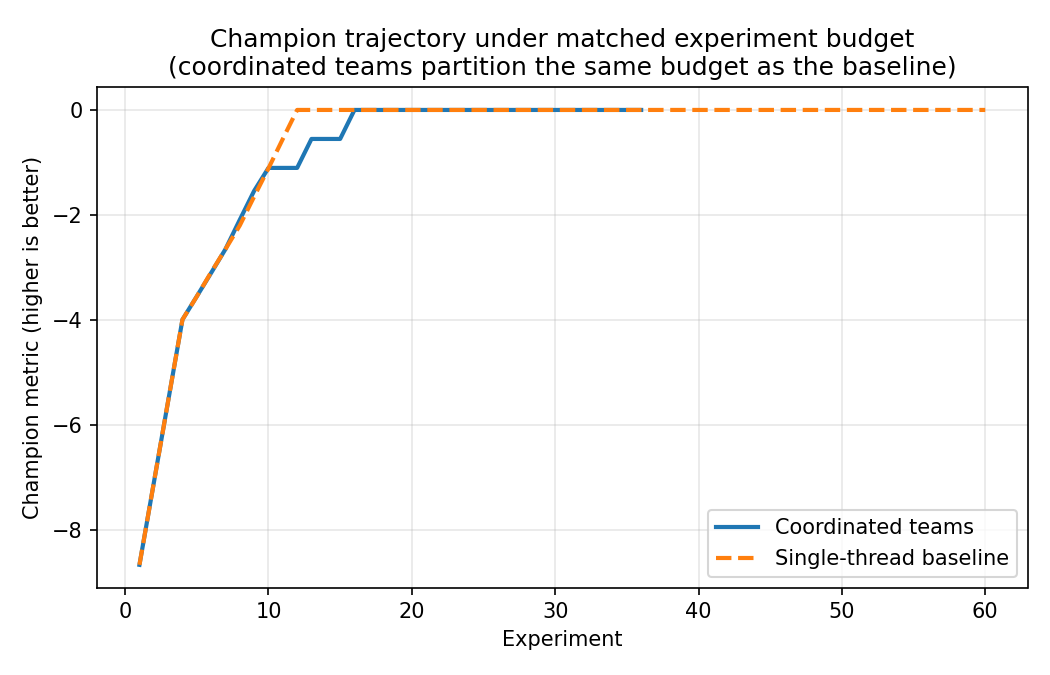
\includegraphics[keepaspectratio,alt={Champion metric (higher is better) versus experiment index for coordinated teams (solid) and the single-thread baseline (dashed) under a matched experiment budget. Coordinated teams partition the same sequential budget as the baseline rather than adding parallel compute, so this is a robustness/efficiency comparison, not a speedup. Produced by run\_search\_comparison.py.}]{../figures/search_comparison.png}}
\caption{Champion metric (higher is better) versus experiment index for
coordinated teams (solid) and the single-thread baseline (dashed) under
a matched experiment budget. Coordinated teams partition the same
sequential budget as the baseline rather than adding parallel compute,
so this is a robustness/efficiency comparison, not a speedup. Produced
by \protect\breaktt{run\_search\_comparison.py}.}\label{fig:comparison}
\end{figure}

The summary in \breaktt{output/data/search\_comparison.json} reports the
decisive quantities:

{\def\LTcaptype{none} % do not increment counter
\begin{longtable}[]{@{}
  >{\raggedright\arraybackslash}p{(\linewidth - 10\tabcolsep) * \real{0.1667}}
  >{\raggedright\arraybackslash}p{(\linewidth - 10\tabcolsep) * \real{0.1667}}
  >{\raggedright\arraybackslash}p{(\linewidth - 10\tabcolsep) * \real{0.1667}}
  >{\raggedright\arraybackslash}p{(\linewidth - 10\tabcolsep) * \real{0.1667}}
  >{\raggedright\arraybackslash}p{(\linewidth - 10\tabcolsep) * \real{0.1667}}
  >{\raggedright\arraybackslash}p{(\linewidth - 10\tabcolsep) * \real{0.1667}}@{}}
\toprule\noalign{}
\begin{minipage}[b]{\linewidth}\raggedright
Configuration
\end{minipage} & \begin{minipage}[b]{\linewidth}\raggedright
Reported metric
\end{minipage} & \begin{minipage}[b]{\linewidth}\raggedright
Clean metric
\end{minipage} & \begin{minipage}[b]{\linewidth}\raggedright
Experiments to optimum
\end{minipage} & \begin{minipage}[b]{\linewidth}\raggedright
Experiments used
\end{minipage} & \begin{minipage}[b]{\linewidth}\raggedright
Redundant re-probes
\end{minipage} \\
\midrule\noalign{}
\endhead
\bottomrule\noalign{}
\endlastfoot
Coordinated teams & \(0.0012\) & \(0.0000\) & \(16\) & \(36\) & \(0\) \\
Single-thread baseline & \(0.0012\) & \(0.0000\) & \(12\) & \(60\) &
\(36\) \\
\end{longtable}
}

Both configurations reach the \textbf{same clean ground-truth optimum}
(\(0.0000\), the global peak), and the clean-metric advantage of
coordination over the baseline is exactly \(0.0000\). This is the honest
headline: under a matched sequential budget, splitting the work into
coordinated teams does \textbf{not} beat the undivided baseline on
solution quality. If anything it is slightly \emph{slower} to first
reach the optimum --- the coordinated run gets there at experiment
\(16\) versus the baseline's \(12\), because partitioning four axes
across three teams interleaves the descent. We make no speedup claim,
because the testbed is constructed so that none would be honest.

What the coordinated configuration \emph{does} gain is \textbf{search
hygiene}: it retires exhausted directions and stops, using only \(36\)
of the \(60\) experiments with zero redundant re-probes, whereas the
baseline --- which runs without the dead-end registry --- spends the
full budget and wastes \(36\) experiments re-testing directions already
known to fail. The coordination machinery changes \emph{how} the budget
is spent, not how good the final answer is.

\subsection{Per-mechanism ablation}\label{per-mechanism-ablation}

The testbed separates two distinct, independently measurable benefits
--- noise robustness and search hygiene --- from the mechanisms that do
not move the needle on this objective. fig.~\ref{fig:ablation} and
fig.~\ref{fig:ablation_efficiency}, drawn from
\breaktt{output/data/ablation.json}, switch off one mechanism at a time
starting from the full coordinated configuration.

\begin{figure}
\centering
\pandocbounded{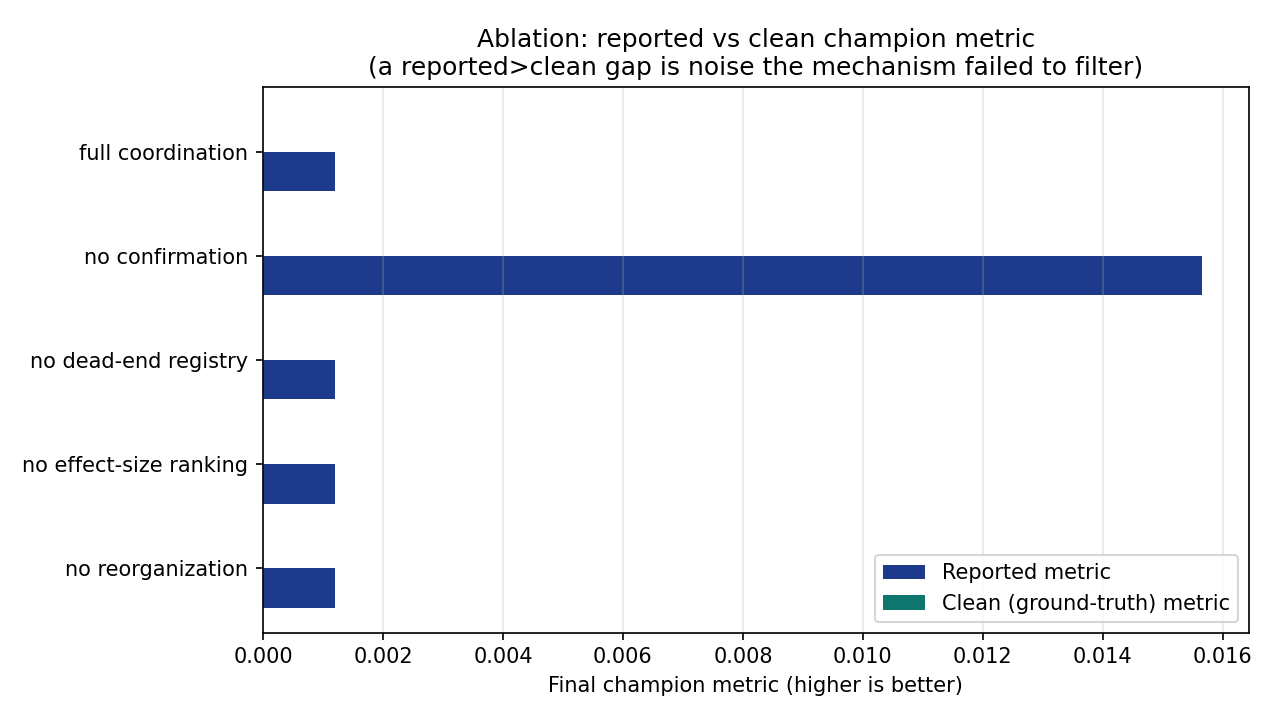
\includegraphics[keepaspectratio,alt={Reported versus clean (ground-truth) champion metric for the full configuration and each single-mechanism ablation. A reported-greater-than-clean gap is accepted noise. Removing noise-band confirmation inflates the gap roughly thirteenfold while the clean metric is unchanged. Produced by run\_ablation.py.}]{../figures/ablation.png}}
\caption{Reported versus clean (ground-truth) champion metric for the
full configuration and each single-mechanism ablation. A
reported-greater-than-clean gap is accepted noise. Removing noise-band
confirmation inflates the gap roughly thirteenfold while the clean
metric is unchanged. Produced by
\protect\texttt{run\_ablation.py}.}\label{fig:ablation}
\end{figure}

{\def\LTcaptype{none} % do not increment counter
\begin{longtable}[]{@{}
  >{\raggedright\arraybackslash}p{(\linewidth - 10\tabcolsep) * \real{0.1667}}
  >{\raggedright\arraybackslash}p{(\linewidth - 10\tabcolsep) * \real{0.1667}}
  >{\raggedright\arraybackslash}p{(\linewidth - 10\tabcolsep) * \real{0.1667}}
  >{\raggedright\arraybackslash}p{(\linewidth - 10\tabcolsep) * \real{0.1667}}
  >{\raggedright\arraybackslash}p{(\linewidth - 10\tabcolsep) * \real{0.1667}}
  >{\raggedright\arraybackslash}p{(\linewidth - 10\tabcolsep) * \real{0.1667}}@{}}
\toprule\noalign{}
\begin{minipage}[b]{\linewidth}\raggedright
Configuration
\end{minipage} & \begin{minipage}[b]{\linewidth}\raggedright
Reported metric
\end{minipage} & \begin{minipage}[b]{\linewidth}\raggedright
Clean metric
\end{minipage} & \begin{minipage}[b]{\linewidth}\raggedright
Noise inflation
\end{minipage} & \begin{minipage}[b]{\linewidth}\raggedright
Experiments used
\end{minipage} & \begin{minipage}[b]{\linewidth}\raggedright
Redundant re-probes
\end{minipage} \\
\midrule\noalign{}
\endhead
\bottomrule\noalign{}
\endlastfoot
Full coordination & \(0.00121\) & \(0.0000\) & \(0.00121\) & \(36\) &
\(0\) \\
No confirmation & \(0.01565\) & \(0.0000\) & \(0.01565\) & \(36\) &
\(0\) \\
No dead-end registry & \(0.00121\) & \(0.0000\) & \(0.00121\) & \(60\) &
\(36\) \\
No effect-size ranking & \(0.00121\) & \(0.0000\) & \(0.00121\) & \(36\)
& \(0\) \\
No reorganization & \(0.00121\) & \(0.0000\) & \(0.00121\) & \(36\) &
\(0\) \\
\end{longtable}
}

\textbf{Confirmation is the load-bearing mechanism for honesty.}
Removing noise-band confirmation leaves the clean metric untouched (the
search still lands on the optimum) but inflates the \emph{reported}
metric from \(0.00121\) to \(0.01565\) --- a roughly \(13\times\)
increase in accepted noise. Without confirmation the search promotes a
champion whose reported value overstates its true value by an order of
magnitude more; with confirmation the reported metric stays close to the
truth. This is exactly the failure mode noise-band confirmation is
designed to prevent, and the testbed measures its size.

\textbf{The dead-end registry is the load-bearing mechanism for
efficiency.} fig.~\ref{fig:ablation_efficiency} shows that removing it
is the only ablation that changes the experiment budget profile: the
registry-consulting proposer otherwise never re-probes a retired
direction (redundant re-probes \(= 0\)) and halts at \(36\) experiments
once every direction is exhausted, while the no-registry configuration
burns all \(60\) experiments and wastes \(36\) of them re-testing known
dead ends. Crucially, this hygiene gain leaves the clean metric
\textbf{unchanged} at \(0.0000\) --- the registry buys a leaner search,
not a better answer.

\begin{figure}
\centering
\pandocbounded{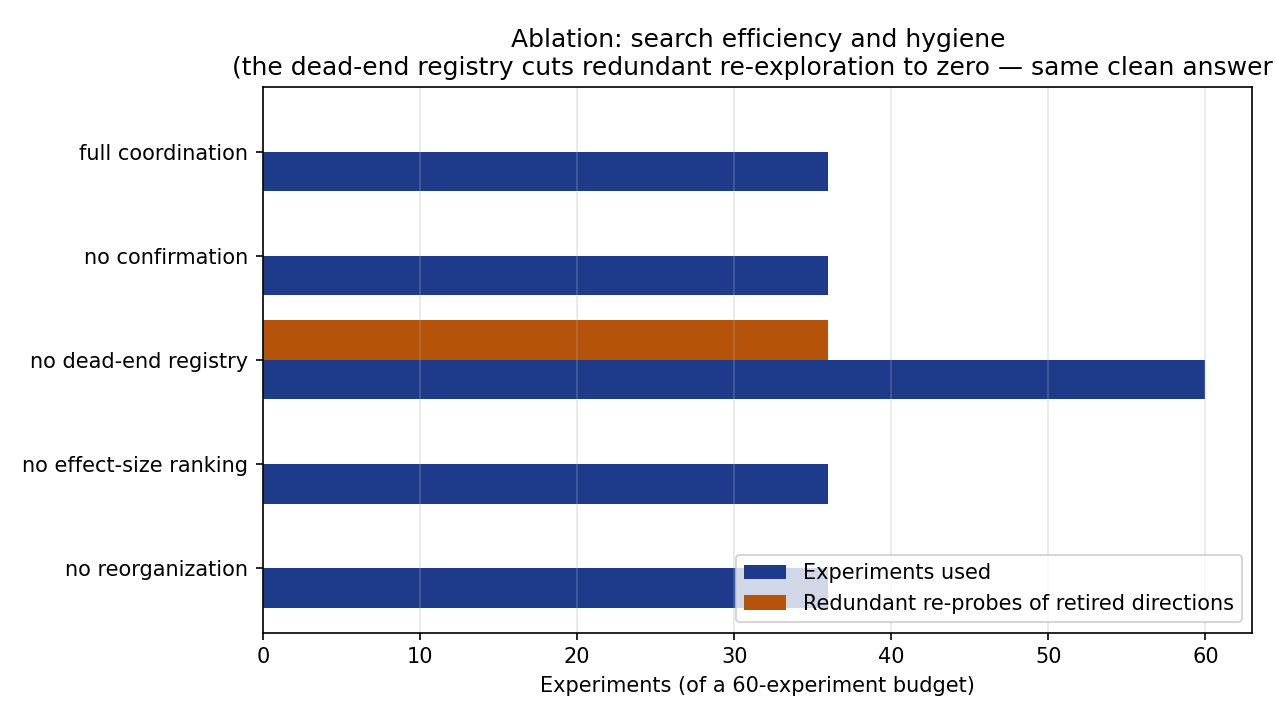
\includegraphics[keepaspectratio,alt={Experiments used and redundant re-probes of retired directions per configuration. Only the dead-end-registry ablation changes the profile: without the registry the search wastes 36 experiments re-exploring known-dead directions and never halts early. Produced by run\_ablation.py.}]{../figures/ablation_efficiency.png}}
\caption{Experiments used and redundant re-probes of retired directions
per configuration. Only the dead-end-registry ablation changes the
profile: without the registry the search wastes \(36\) experiments
re-exploring known-dead directions and never halts early. Produced by
\protect\texttt{run\_ablation.py}.}\label{fig:ablation_efficiency}
\end{figure}

\textbf{Effect-size ranking and reorganization do not move any metric
here.} Removing either leaves the reported metric, clean metric,
experiments used, and redundant re-probes all unchanged. On this small,
separable objective with a deterministic proposer, those two mechanisms
reshape the \emph{order} in which directions are tried without changing
the destination, the noise, or the efficiency within the budget. We
report this plainly rather than dressing it up: both are correctly
implemented and independently tested, but their benefit is about
exploration bookkeeping on harder or more deceptive landscapes, not
about measurable gains on this testbed.

\subsection{What the numbers say}\label{what-the-numbers-say}

Four honest conclusions follow directly from the data:

\begin{enumerate}
\def\labelenumi{\arabic{enumi}.}
\tightlist
\item
  Under a matched budget, coordinated teams neither beat nor lose to the
  single-thread baseline on clean solution quality (advantage
  \(= 0.0000\)), and partitioning is in fact marginally slower to first
  reach the optimum (\(16\) vs \(12\) experiments).
\item
  Noise-band confirmation delivers a measurable, reproducible robustness
  benefit: a \(\sim 13\times\) reduction in accepted noise
  (\(0.01565 \to 0.00121\) reported-vs-clean gap).
\item
  The dead-end registry delivers a measurable efficiency benefit:
  redundant re-probes fall from \(36\) to \(0\) and the search halts at
  \(36\) rather than \(60\) experiments --- with the clean answer
  unchanged.
\item
  Effect-size ranking and reorganization are correctly implemented and
  ablatable, but do not by themselves change any measured quantity on
  this objective --- a result we report rather than obscure.
\end{enumerate}

\newpage

\section{Experimental Setup}\label{sec:setup}

\subsection{Objective and budget}\label{objective-and-budget}

All experiments optimize the synthetic objective of
sec.~\ref{sec:methodology} with \(d = 4\) dimensions, ripple amplitude
\(\rho = 0.15\), and per-evaluation noise scale
\(\sigma_{\text{noise}} = 0.02\). The global optimum is the origin,
where the clean objective equals \(0\). Every configuration is given the
\textbf{same} budget of \(60\) sequential experiments; coordinated
configurations partition that budget across teams.

\subsection{Configurations}\label{configurations}

The configurations compared in sec.~\ref{sec:results} correspond
directly to \texttt{SearchConfig} objects:

\begin{itemize}
\tightlist
\item
  \textbf{Coordinated teams} --- the full configuration: \(3\) teams,
  all mechanisms on (\breaktt{use\_confirmation},
  \texttt{use\_dead\_ends}, \texttt{use\_ranking},
  \breaktt{use\_reorganization} all true).
\item
  \textbf{Single-thread baseline} ---
  \breaktt{SearchConfig.single\_thread\_baseline()}: \(1\) team,
  confirmation on (so the baseline is itself noise-honest), all
  structural coordination off.
\item
  \textbf{Ablations} --- the full configuration with exactly one
  mechanism switched off, generated via \breaktt{dataclasses.replace}.
\end{itemize}

Confirmation averages each candidate over seeds \((101, 202, 303)\) and
tests against a \(\sigma = 2\) noise band; the primary evaluation seed
is \(7\); the stagnation window is \(10\) experiments; a direction is
retired after \(3\) consecutive non-improving experiments. These values
are the \texttt{SearchConfig} defaults and are echoed in
\breaktt{manuscript/config.yaml}.

\subsection{Proposer}\label{proposer}

The rendered figures and the JSON summaries are produced with
\breaktt{DeterministicProposer}, a rule-based agent that reads the shared
state and emits a concrete proposal. No mock objects are used anywhere.
The live \texttt{HermesProposer} path is not part of the rendered
pipeline; it is exercised separately (see
sec.~\ref{sec:reproducibility}).

\subsection{Outputs}\label{outputs}

Two thin orchestrator scripts produce all results:

\begin{itemize}
\tightlist
\item
  \breaktt{scripts/run\_search\_comparison.py} \texorpdfstring{\ensuremath{\to}}{->}
  \breaktt{../figures/search\_comparison.png},
  \breaktt{output/data/search\_comparison.json}.
\item
  \breaktt{scripts/run\_ablation.py} \texorpdfstring{\ensuremath{\to}}{->} \breaktt{../figures/ablation.png},
  \breaktt{output/data/ablation.json}.
\end{itemize}

Each script imports all computation from \texttt{src/}, runs the
configurations, and writes a figure plus a machine-readable summary. The
numbers quoted in sec.~\ref{sec:results} are read directly from those
JSON files.

\newpage

\section{Reproducibility}\label{sec:reproducibility}

Every figure and number in this manuscript is regenerable from a clean
checkout with fixed seeds and no network access.

\subsection{Deterministic core}\label{deterministic-core}

The objective is a pure function of \texttt{(params,\ seed)}, and the
coordination loop is deterministic given the objective, proposer, and
configuration. Re-running the analysis scripts reproduces the figures
and the JSON summaries byte-for-byte.

\begin{Shaded}
\begin{Highlighting}[]
\CommentTok{\# Regenerate the matched{-}budget comparison and the ablation}
\ExtensionTok{uv}\NormalTok{ run python projects/templates/template\_autoscientists/scripts/run\_search\_comparison.py}
\ExtensionTok{uv}\NormalTok{ run python projects/templates/template\_autoscientists/scripts/run\_ablation.py}
\end{Highlighting}
\end{Shaded}

\subsection{Tests and coverage}\label{tests-and-coverage}

The project carries its own test suite under \texttt{tests/}, run as a
standalone per-project gate. There are no mocks anywhere: the
\breaktt{DeterministicProposer}, the synthetic objective, and the
registries are all real objects exercised with real numerical inputs.

\begin{Shaded}
\begin{Highlighting}[]
\CommentTok{\# Project test suite with the per{-}project coverage gate}
\ExtensionTok{uv}\NormalTok{ run pytest projects/templates/template\_autoscientists/tests/ }\DataTypeTok{\textbackslash{}}
    \AttributeTok{{-}{-}cov}\OperatorTok{=}\NormalTok{projects/templates/template\_autoscientists/src }\AttributeTok{{-}{-}cov{-}fail{-}under}\OperatorTok{=}\NormalTok{90}
\end{Highlighting}
\end{Shaded}

The deterministic core is tested to full coverage. The live
language-model path is excluded from the coverage gate
(\breaktt{\#\ pragma:\ no\ cover}) because it requires an external
service.

\subsection{The live Hermes agent
(opt-in)}\label{the-live-hermes-agent-opt-in}

\texttt{HermesProposer} calls a Hermes model served by Ollama. It is not
part of the rendered pipeline and is exercised only by an opt-in test
marked \texttt{requires\_ollama}:

\begin{Shaded}
\begin{Highlighting}[]
\CommentTok{\# One{-}time: start Ollama and pull a Hermes model}
\ExtensionTok{ollama}\NormalTok{ serve}
\ExtensionTok{ollama}\NormalTok{ pull hermes3}

\CommentTok{\# Run the live round{-}trip test}
\ExtensionTok{uv}\NormalTok{ run pytest projects/templates/template\_autoscientists/tests/test\_hermes\_live.py }\DataTypeTok{\textbackslash{}}
    \AttributeTok{{-}m}\NormalTok{ requires\_ollama }\AttributeTok{{-}v}
\end{Highlighting}
\end{Shaded}

Because the loop depends only on the \texttt{Proposer} protocol,
swapping \breaktt{DeterministicProposer} for \texttt{HermesProposer} is
the single change needed to turn the reproducible reference run into a
live agentic one --- the coordination mechanisms, ablation toggles, and
confirmation logic are unchanged.

\subsection{Shared estimator}\label{shared-estimator}

The noise-band confirmation estimator is generic. A synchronized copy
lives at \breaktt{infrastructure.scientific.confirmation}
(\breaktt{confirm\_improvement}, \texttt{Confirmation}) for reuse by any
other project that compares a stochastic metric to a baseline, and is
covered by \breaktt{tests/infra\_tests/scientific/test\_confirmation.py}.
The project keeps its own standalone copy so the exemplar runs
self-contained.

\newpage

\section{Scope and Related Work}\label{sec:scope}

\subsection{What this exemplar claims}\label{what-this-exemplar-claims}

\begin{itemize}
\tightlist
\item
  The five AutoScientists coordination mechanisms
  \citep{gao2026autoscientists} are re-implemented faithfully enough to
  be \textbf{individually ablatable}, and each is independently tested.
\item
  Under a \textbf{matched sequential experiment budget}, coordinated
  teams reach the same clean optimum as a single-thread baseline
  (advantage \(= 0.0000\)).
\item
  \textbf{Noise-band confirmation} produces a measurable, reproducible
  reduction in accepted evaluation noise (a \(\sim 13\times\) smaller
  reported-vs-clean gap on this objective).
\item
  The \textbf{dead-end registry} produces a measurable, reproducible
  search-hygiene gain: consulted by the proposer, it cuts redundant
  re-probes of retired directions from \(36\) to \(0\) and halts the
  search at \(36\) of \(60\) experiments, with the clean optimum
  unchanged.
\item
  The \textbf{language-model proposer is a clean plug-in seam}: a live
  Hermes agent can replace the deterministic proposer without changing
  the coordination loop.
\end{itemize}

\subsection{\texorpdfstring{What this exemplar does \emph{not}
claim}{What this exemplar does not claim}}\label{what-this-exemplar-does-not-claim}

\begin{itemize}
\tightlist
\item
  \textbf{No speedup.} Because coordinated teams partition one budget
  rather than adding parallel compute, this testbed is not evidence that
  coordination is faster or reaches better solutions. It is constructed
  so that no such claim would be honest, and the measured advantage is
  zero.
\item
  \textbf{No generalization of the magnitudes.} The \(\sim 13\times\)
  noise-reduction figure, the \(36 \to 0\) redundancy reduction, and the
  null effect of effect-size ranking and reorganization on every
  measured quantity are properties of \emph{this} synthetic objective,
  budget, and deterministic proposer. They illustrate the measurement,
  not a universal constant.
\item
  \textbf{No agentic-quality claim.} The live Hermes path demonstrates
  that the seam works, not that an LLM proposer outperforms the
  rule-based one.
\end{itemize}

\subsection{Relationship to
AutoScientists}\label{relationship-to-autoscientists}

The original system \citep{gao2026autoscientists} runs real
language-model agent teams on real, expensive scientific tasks and
reports end-to-end performance. This exemplar deliberately strips that
to a deterministic core so the \emph{mechanisms} can be attributed and
the noise behavior measured in isolation. It is a complement --- a
microscope on the coordination primitives --- not a reproduction of the
full system or its empirical results.

\subsection{Related context}\label{related-context}

The confirmation mechanism is an application of standard effect-size and
standard-error reasoning \citep{cohen1988statistical} to online
acceptance decisions. The dead-end registry, effect-size ranking, and
reorganization are coordination heuristics whose lineage runs through
population- and restart-based search \citep{whitley2001overview}; the
contribution here is not the heuristics but their honest, ablatable
measurement. The broader setting --- teams of language-model agents
pursuing a long-running objective --- sits within the rapidly growing
literature on LLM-based autonomous agents \citep{wang2023survey}.
Throughout, the emphasis on regenerable figures, fixed seeds, and a
tested core follows the reproducible-research tradition
\citep{peng2011reproducible}.

\newpage

\section{Conclusion}\label{sec:conclusion}

This exemplar re-implements the AutoScientists coordination mechanisms
\citep{gao2026autoscientists} as a deterministic, ablatable testbed and
reports what they actually do under a fair, matched experiment budget.
The central methodological commitment is honesty about the comparison:
coordinated teams partition one sequential budget rather than adding
parallel compute, so we neither expect nor observe a speedup, and we say
so. The clean-metric advantage of coordination over a single-thread
baseline is exactly zero.

Two results are worth keeping. The first is the noise-robustness
measurement: by separating the reported champion metric from the clean
ground-truth metric --- possible only because the objective is synthetic
--- the testbed quantifies noise-band confirmation as a roughly
thirteenfold reduction in accepted noise, with the clean optimum reached
either way. The second is search hygiene: the dead-end registry,
consulted by the proposer, drives redundant re-probes of retired
directions from \(36\) to \(0\) and lets the search halt at \(36\) of
the \(60\) experiments instead of burning the full budget --- without
changing the clean answer. The remaining structural mechanisms
(effect-size ranking, stagnation reorganization) are correctly
implemented and independently testable, but on this separable objective
they reshape the search path without changing its destination, noise, or
efficiency within the budget; we report that rather than overstate it.

Two properties make the artifact reusable. First, every mechanism is
gated behind a single configuration object, so the ablation is a clean
subtraction and the testbed extends naturally to harder objectives where
the structural mechanisms have more to do. Second, the language-model
proposer is a genuine plug-in seam: the deterministic proposer drives
the reproducible figures, and a live Hermes agent can replace it without
touching the coordination loop. The honest-testbed framing is the
contribution --- a small, fully reproducible instrument for attributing
coordination effects to mechanisms and for distinguishing real gains
from noise.

\newpage

\section{References}\label{sec:references}

Bibliography lives in
\href{references.bib}{\breaktt{manuscript/references.bib}} and is read by
Pandoc during PDF render. The build pipeline invokes Pandoc with
\texttt{-\/-natbib}, so every \texttt{{[}@key{]}} citation in the
manuscript is rewritten to the appropriate
\texttt{\textbackslash{}cite\{\}}/\texttt{\textbackslash{}citep\{\}}/\texttt{\textbackslash{}citet\{\}}
LaTeX command and resolved against the bib file.

To validate that \texttt{references.bib} is syntactically clean and
contains the required fields per entry type:

\begin{Shaded}
\begin{Highlighting}[]
\ExtensionTok{uv}\NormalTok{ run python }\AttributeTok{{-}m}\NormalTok{ infrastructure.reference.citation.cli validate }\DataTypeTok{\textbackslash{}}
\NormalTok{    projects/templates/template\_autoscientists/manuscript/references.bib }\AttributeTok{{-}{-}strict}
\end{Highlighting}
\end{Shaded}




\clearpage

\bibliography{references}
\end{document}
